\section{Logical Agents}
Humans do things based of the process of reasoning that operate on internal representations of knowledge, in AI, reasoning is embodied in knowledge-based agents \cite[Chapter 7]{russell2016artificial}. When states are only partially observable, i.e, the agents information set is not trivial, the agent must explore all possibilities before moving. With the development of heuristics and the use of some knowledge-base, the agent can act with a sense of logic. This project focuses on knowledge-based agents without additional mechanisms that provide learning.\\

\noindent A well made knowledge-based agent can be designed by giving it a sequence of actions or procedures to follow, with a combination of statements telling the agent how to follow them. \cite[Chapter 7]{russell2016artificial} These are included within the agent's knowledge base. We can construct these sentences in propositional logic. A sentence is constructed from atomic sentences and complex sentences, where atomic sentences consist of a single proposition symbol i.e $\top$ (True), $\bot$ (False), $P$, $Q$, etc; and complex sentences are comprised of atomic sentences and connectives. For example, in a knowledge-base with two propositional letters $p$ and $q$, the 4 connectives to note \cite[Chapter 7]{russell2016artificial} used in this report are:

\begin{itemize}
    \item $\neg p$ (not p), $\neg$ flips the truth value of $p$
    \item $p \land q$ (p and q), $\land$ is the symbol for a conjunction, both $p$ and $q$ must be $\top$ for $p \land q$ to be $\top$ 
    \item $p \lor q$ (p or q), $\lor$ is the symbol for a disjunction, either $p$ or $q$ must be $\top$ for $p \lor q$ to be $\top$
    \item $p \rightarrow q$ (p or q), $\rightarrow$ represents an implication, it is usually read as: if $p$, then $q$. $p \rightarrow q$ is only $\bot$ if $p = \top$ and $q = \bot$ 
\end{itemize}

\noindent These propositional letters are used to define situations in the environment. For example, in the knowledge-base of an agent, $p_{x, y}$ would be $\top$ if the agent is at position $(1, 0)$ in the environment. The procedures and actions are used to set the truth value of these predicates. Further explanations of this are given in the following section.

\newpage
\subsection{Logical Inference and Plans}
After the construction of the agents knowledge-base $KB$, we want to determine whether the agent can arrive at some conclusion $\alpha$ in a finite number of steps. I.e. can the agent reach some goal state given $KB$? Formally this problem is written as $KB \models \alpha$. This has been proven to be decidable by the works of Godel and Turing \cite[Chapter 7]{russell2016artificial}. A plan is defined as a sequence of actions that lead to the solution of the goals set in an environment. These actions must declare what variables change and what stays the same in its definition \cite[Chapter 7]{russell2016artificial}.

\begin{itemize}
    \item The initial definition of states.
    \item The successor-state axioms for all possible actions at each time up to some maximum time $t$. In this report, we assume that an action takes up 1 unit of time.
    \item The assertion that the goal is achievable at time $t$, i.e $\alpha^t = \top$
\end{itemize}

\noindent After generating this sentence, if there exists some assignment of truth values to the variables in the sentence such that the sentence resolves to $\top$. We can extract those variables in the sentence that are assigned to $\top$. This represents a plan that achieves the goal $\alpha$. \cite[Chapter 7]{russell2016artificial} This truth assignment can be found through truth table look-ups or logical inference rules, that isn't covered in this report, however in problems with complex environments, this becomes significantly more computationally complex to compute. For example, using propositional inference, generating a sentence to prove that the agent can reach all locations would involve observing every location, in every orientation available to the agent. When looking at situations where the agent must avoid locations or collect items, it can be seen that this would become very costly.

\section{Classical Planning}
Due to the limitations of these hybrid propositional logic agents on complex environments, classical planning was developed to devise a faster method of generating plans to reach a goal. The agent's $KB$ is instead modelled as a problem that consists of first-order-logic and action schema. \cite[Chapter 10]{russell2016artificial} Classical planning is the successor to STRIPS planning which used the notion of knowledge-based agents. \cite{suárezhernández2021strips}

\subsection{First-Order Logic}
Propositional logic focuses on the truth relation between sentences and possible worlds, which lacks the expressive capability to describe an environment with many objects. \cite[Chapter 8]{russell2016artificial} For example to write the statement: "the box is on the floor" is very difficult using propositional sentences. First-order-logic is built around more complex relationships between objects in an environment, instead of simply stating that whether or not something exists within the environment \cite[Chapter 8]{russell2016artificial}.

\subsubsection{Domains}
The domain of a first-order logic model is the set of objects or domain elements that it contains \cite[Chapter 8]{russell2016artificial}. In this report, we deal with non-empty domains, every environment must contain at least one thing that can be expressed or described. These objects may have some relation. For example, in an environment with a table and floor we could see the mappings: \[(table \rightarrow position), (floor \rightarrow position)\]

\subsubsection{Definitions (Predicates, Fluents, Objects and Quantifiers)}
In first-order logic, we write relations using predicate symbols. The example statement can be expressed in first-order logic as the predicate: $On(box, floor)$, where $On$ is the predicate symbol; $box$ and $floor$ are the objects. A predicate has a fixed number of arguments that returns either $\top$ or $\bot$. A fluent is a condition that can change over time, as we model actions that take up a constant unit of time, we define fluents as a statement containing a predicate and its truth value. For example, if in our environment the box is on the floor then a fluent in the agent's knowledge-base would be: $On(box, floor) = \top$. First-order logic statements can also be quantified, for example, to state that all objects $x$ in our domain are positions, we would write the expression: $\forall x, (x \rightarrow position)$.  $\forall$ means "for all" and $\exists$ means "there exists". \cite[Chapter 8]{russell2016artificial}

\subsection{Planning Domain Definition Language (PDDL)}
In response to the limitations imposed by propositional inference based agents, planning researchers, notably Drew McDermott developed a factored representation in which the state of an environment is represented by a collection of variables. This family of languages is called the Planning Domain Definition Language (PDDL). \cite{ghallab_pddl_1998} This report focuses on PDDL1.2 which focuses on a primarily predicate way of modelling. PDDL requires four things to define a state search problem, three of which are used in the generation of sentences in plan synthesis mentioned in the previous section. The requirement for successor-state axioms is split into two parts: the actions available within a state and the result of applying an action. A state is represented as a conjunction of fluents, for example if the box is on the floor and there is a bear on the table, we can model this as: $On(box, floor) \land On(bear, table)$. States cannot contain fluents that contain variables or functions, they must be ground \cite[Chapter 10]{russell2016artificial}, for example $At(x)$ is not allowed if $x$ can vary at that state.

\subsubsection{Action Schema}
In PDDL, actions are described by a set of action schema, each action contains a precondition and an effect. The precondition is a sentence that must return $\top$ before the effect is evaluated. The effect sets the given sentence to $\top$. For example, below is action schema that moves the tells the agent to move an object $object$ from position $from$ to position $to$ in first-order logic \cite[Chapter 10]{russell2016artificial}: 

\begin{align*}
    Acti&on(move(object, to, from),\\
        &\text{\textsc{Precondition:}}\: At(object, to) \land Path(to, from)\\
        &\text{\textsc{Effect:}}\: At(object, from))
\end{align*}
\newpage

\noindent In PDDL the $move(object, to, from)$ action is shown below in Figure 2.1:

\begin{figure}[h!]
\centering
\begin{BVerbatim}
(:action move
    :parameters (?object ?to ?from)
    :precondition (and (at ?object ?to) (path ?to ?from))
    :effect (and (at ?object ?from))
)
\end{BVerbatim}
\caption{PDDL Action Example}
\end{figure}

\noindent The precondition occurs at time $t$ and the effect occurs at time $t+1$. An action $a$ can be executed in some state $s$ if $s \models Precondition(a)$ \cite[Chapter 10]{russell2016artificial}. 

\subsubsection{Planning Domains and Problems}
The set of action schemas is defined within the planning domain, along with types, constants and available predicates in the knowledge-base. The planning problem contains the initial truth values of fluents from predicates in the domain; objects, and the goal state $\alpha$ \cite{ghallab_pddl_1998}. Examples of these are covered within the Design section of this report. To note: this report focuses on the agent having full state observability and the actions in the domain are all deterministic, i.e there the result of an action can be determined.

\subsubsection{Formalism}
In this report, a classical planning instance (known as a PDDL problem) is the quadruple $P = \langle X, A, I, G \rangle$. where \cite{segovia-aguas_generalized_2021}:
\begin{itemize}
    \item $X$ is the set of state variables, which is the set of all possible predicates. As mentioned previously a state is the conjunction of fluents, this can also be described as: $x \in X$ $s_t = \langle x_0 = v_0, ..., x_{|X|} = v_{|X|} \rangle$ where $v_k$ is the truth value assigned to the predicate $x_k$ and $s_t \in S$ is the state observed at time $t$. $X$ must be non-empty as it describes the environment defined within a problem.
    \item $A$ is the set of action schema
    \item $I$ is the initial state, $I \in S$ 
    \item $G$ is a goal condition on the state variables $X$ that induces a set of goal states $S_G$ that is a subset of $S$, $S_G = \{s \mid s \models G, s \in S\}$.
\end{itemize}

\noindent A plan $\pi = \langle a_1, ..., a_m \rangle, a_i \in A$ \textit{solves} $P$ if the execution of $\pi$ with $s_0 = I$ finishes in a goal state $s_m \in S_G$ for some $m \leq |S_G|$. The plan $\pi$ is \textit{optimal} if $|\pi|$ is minimal amongst the plans that solve the problem $P$. In this report, the \textit{cost} of generating $\pi$ is $|\pi|$ \cite{segovia-aguas_generalized_2021}.

\subsection{Fast Downward}
Fast Downward is a classical planning system, designed specifically for solving deterministic planning problems. It employs a forward heuristic search methodology \cite{heuristicplanning}, to navigate through the state space. This methodology yields low-cost plans that are efficienctly discovered \cite{helmert_fast_2006}.  Fast Downward is authored notably by Malte Helmert, and has received contributions from numerous researchers and developers over the years, maintaining its relevancy in modern classical planning. The planner is renowned for its performance and adaptability. Fast Downward utilizes heuristics to navigate through the state space. \cite{helmert_fast_2006}. In the 9th International Planning Competition (IPC), Fast Downward was utilized by two winning planners \cite{vie2022adversarial}. Its performance in the IPC shows its capability to find optimal or near-optimal plans within specified time constraints. Fast Downward serves as the classical planner used in the synthesis of all classical planning instances within this project.

\section{Generalised Planning}
Generalised planning is a shift in focus away from generating plans quickly, but instead focuses on the structure of the plan generated. Generalised planning attempts to synthesise a plan over a set of classical planning instances $\mathcal{P}$, where $|\mathcal{P}| \geq 1$. These instances are all problems that share the same domain. A generalised plan has an algorithm-like solution that is valid over $\mathcal{P}$. \cite{jimenez_review_2019} The algorithm produced can be in a variety of theories/languages. In this report, generalised solutions are produced in a C++ manner, utilising pointers and control flow structures \cite{segovia-aguas_representation_2022}. Furthermore, a generalised plan is a generative model, a top-down approach begins with an empty program of set length, and iteratively generates lines of the algorithm until a solution is found that solves all the planning instances \cite{jimenez_review_2019}. The generalised plan can then be used to generate the classical plans for each planning instance \cite{jimenez_review_2019}. Due to the nature of this task, generalised planning is computationally expensive, taking exponentially more time in the worst case than classical planning. The upper bound on the number of actions is given by the total number of possible states of the generalised plan \cite{backstrom_automaton_plans}. 

\subsection{Best First Search Generalised Planning (BFGP)}
Due to the complexity of generalised planning, researchers (Javier, Sergio, Angers) have developed methods to find generalised plans in a much more reasonable time frame through optimising classical planning, alongside the well-known Best First Search (BFS) algorithm \cite{segovia-aguas_generalized_2021}.

\subsubsection{Planning with Pointers}
The planning model is extended with the use of a memory unit that contains $|Z| + 2$ pointers. This allows for powerful memory management so that reusing defined state variables across $\mathcal{P}$ takes up less space in actual memory. The $Z$ pointers reference the original planning state variables, in the memory unit. The other two pointers are zero and carry bit flags. For a classical planning instance $P = \langle X, A, I, G \rangle$, the extended model with registers is defined by $P_Z =\langle X_Z', A_Z', I_Z', G \rangle$ where \cite{segovia-aguas_generalized_2021}:

\begin{itemize}
    \item $X_Z' = X \cup \{y_z, y_c\} \cup Z$, where $\{y_z, y_c\}$ are the respective flags and $Z$ is the non-empty set of pointers of length $|X|$.
    \item $A_Z' = A' \cup R_Z$, where $A'$ is the set of action schema $A$ that uses pointers as parameters instead of objects. The set $R_Z = \{inc(z1), dec(z1), cmp(z1, z2), cmp(\text{*} z1, \text{*} z2), \\set(z1, z2) \mid z1, z2 \in Z\}$ is the set of actions that modify some pointers $z1, z2 \in Z$. 
    \item $I_Z'$ is the same initial state as defined by $I$, with the addition of $y_z = \bot, y_c = \bot$
\end{itemize}

\noindent A generalised plan is defined by $\Pi = \langle a_1, ..., a_m, end \rangle,\, a_i \in A_Z$. $\Pi$ can contain $goto$ instructions that reference another program line in the program, and the final element of $\Pi$ is always $end$. $\Pi$ solves $\mathcal{P}$ if there execution of all plans $\pi_i, (1 \leq 0 \leq |P|) $ generated by the algorithm described in $\Pi$ solves $P_i \in \mathcal{P}$. The \textit{cost} of $\Pi$, given by the sum of the length of the classical plans. The emprical performance measure is important within experiments in this report when we look at the FastDownward's plan synthesis in comparison to the solutions generated by BFGP \cite{segovia-aguas_generalized_2021}.

\subsubsection{Evaluation and Heuristics}
The evaluation is taken over a set of functions $f(\Pi)$ where $\Pi$ is a \textit{partially specified} generalised plan. In this report, a partially specified generalised plan is an incomplete generalised plan where the the full algorithm that solves all the planning instances has not been generated fully. This evaluation score yields stronger positive values as it $\Pi$ gets closer to solving all problems in $\mathcal{P}$. In this planner, the evaluation is done by observing the plan structure, measuring the number of $goto$, unused and repeated instructions in $\Pi$ \cite{segovia-aguas_generalized_2021}.

\subsubsection{Algorithm}
BFGP sequentially expands to the state that is optimal in a priority queue of states sorted based on the scores given by the evaluation and heuristic functions. If the execution of $\Pi$ fails during the execution of these functions, i.e due to infinite loops or there not being enough program lines available to represent the generalise plan, then that state is a \textit{dead-end} and is not explored. If $\Pi$ solves all instances in $\mathcal{P}$, then the solution is valid, and the algorithm terminates \cite{segovia-aguas_generalized_2021}.

\subsubsection{Example Plan}
Below is an example output $\Pi$ generated by the BFGP algorithm, using C++ theory.
\begin{figure}[h!]
\centering
\begin{BVerbatim}
0. for(ptr_position_0++,8)
1. for(ptr_position_1++,3)
2. move(ptr_position_0,ptr_position_1)
3. endfor(ptr_position_1++,1)
4. for(ptr_position_1--,7)
5. move(ptr_position_1,ptr_position_0)
6. move(ptr_position_0,ptr_position_1)
7. endfor(ptr_position_1--,4)
8. endfor(ptr_position_0++,0)
9. end
\end{BVerbatim}
\caption{BFGP++ Plan Example}
\end{figure}
\\The \texttt{for}($z$, $i$) statement modifies the pointer $z$ an arbitrary number of times, that differs from classical plan to plan. ++ calls $inc(z)$ which increments the pointer $z$ and -- calls $dec(z)$, which decrements the pointer $z$. On each modification, it executes the actions constrained between its current instruction line and the the $i$th instruction line.

\section{Complex Path Finding Games}
In this report, we refer to \textit{complex path finding games} as games that contain more complexity than an action that causes the agent to move from one position to the next. In these games the agent must navigate through an environment to reach a goal destination. Due to the popularity of these problems in research, a lot of games of this style have been produced over many years. This project focuses on two well-known games of this style: Maze and Snake.

\subsection{Maze}
Mazes involve an environment that contains a set of locations called a board, a start position and a goal position. The locations are blocked off by walls that stop the agent from moving from one location to another in a specific direction. In this project, we look at mazes in which sections of the board are removed from the environment completely. Blockly Games is a series of educational games designed to teach programming concepts using a block-based interface. This section focuses on the Maze game, in which the user must select a series of code-blocks to make the player reach the goal. There are 10 levels that are increasing in difficulty which contain conditional statements and iteration.

\begin{figure}[h!]
\centering
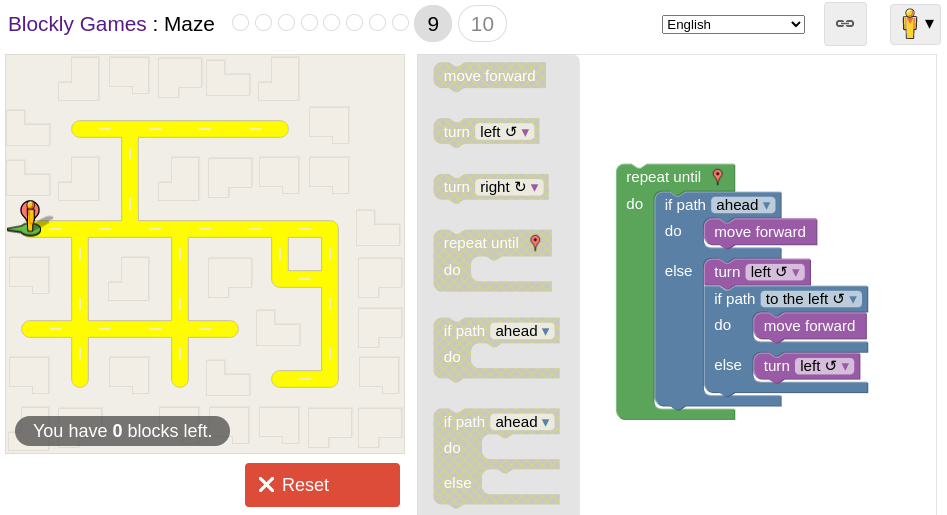
\includegraphics[width=\textwidth]{images/blockly_maze.png}
\caption{Solution to level 9 of Blockly Games: Maze}
\end{figure}

\noindent The yellow locations are locations that the agent can traverse. The agent is represented by a yellow figure on a green arrow, and the goal is the red marker. In this project, the focus is on the three core code-blocks: 
\begin{itemize}
    \item Move forward - the agent can move in the direction of the green marker by one unit
    \item Move left/right - the agent can turn left or right by 90\degree.
\end{itemize}
The notion of orientation adds extra complexity to the solution generated by the generalised planner. Due to the difficulty of formalising control flow statements into PDDL, this report will not cover them. Furthermore, this report will look at a large variety of problems outside of the 10 listed in the Blockly Games: Maze collection.

\subsection{Snake}
Snake is a well known classical digital game in which the player controls the agent, also known as the "snake", to maximise their score by eating "apples" generated at random locations. As the snake consumes apples, it grows in length occupying a position behind the snake permanently. Below is an example of the snake environment:\\

\begin{figure}[h!]
\centering
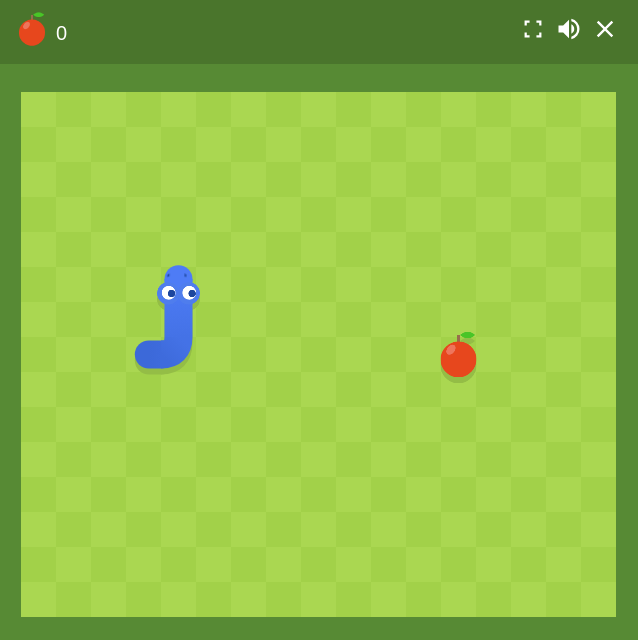
\includegraphics[width=0.5\textwidth]{images/google_snake.png}
\caption{Google's Snake game.}
\end{figure}

\noindent Avoiding collisions is key to survival, consuming itself or coming in contact with the border kills the snake. In the video game, the snake can consume apples endlessly until its body fills up the board, however, in the domain defined in the Design section, the snake's goal is to collect all the available apples set in the problem. This domain is significantly more complex than the maze problems due to the extra goals and conditions set on the agent, leading to very extensive state spaces. Although this domain is created optimally, the generalised planner struggles to compile a solution even for the most basic problems, hence this development of plans will focused more primarily on classical planning and solutions generated on problems with this domain.